%%% Local Variables:
%%% mode: latex
%%% TeX-master: "../frankfurt"
%%% End:

\subsection{}
\begin{frame}
  \frametitle{Karger's Algorithm}
\only<1>{
      \begin{itemize}
    \item Contraction method is used.
      \item Randomized selection of Edges.
        \item Running multiple times of the algorithm will provide
          more accurate result.
    \end{itemize}
}

\only<2>{
  \begin{itemize}
\item Basically one run of Karger's Algo takes {\bf $O(n^2)$} time.
\item It achieves error probability of $\frac{1}{poly(n)}$ with
  $O(n^4\log{}n)$ time.
  \end{itemize}

Derivation will be given in the later part.
}
\only<3>{


}

\end{frame}


\begin{frame}
  \frametitle{Algorithm}
\only<1>{

\begin{greenblock}{Karger's Algorithm:}
      \begin{algorithm}[H]
        \small
        Given $\xk{0} \in \dom f$\;
        \Repeat{stopping criterion is satisfied}{
          Determine a descent direction $\Delta x$ $\Rightarrow$
          {$\footnotesize Gradient/Steepest Descent$}\;
          Choose a step size $t > 0$ $\Rightarrow$~~~~~~~~~~~~ $Line Search Algo$ \;
          Update $x := x + t \Delta x$\;
        }
        % \caption{Descent Method Algorithm}
      \end{algorithm}
    \end{greenblock}


}
\end{frame}

\begin{frame}
  \frametitle{Results}

\vspace*{-1.5cm}
  \hspace*{2cm}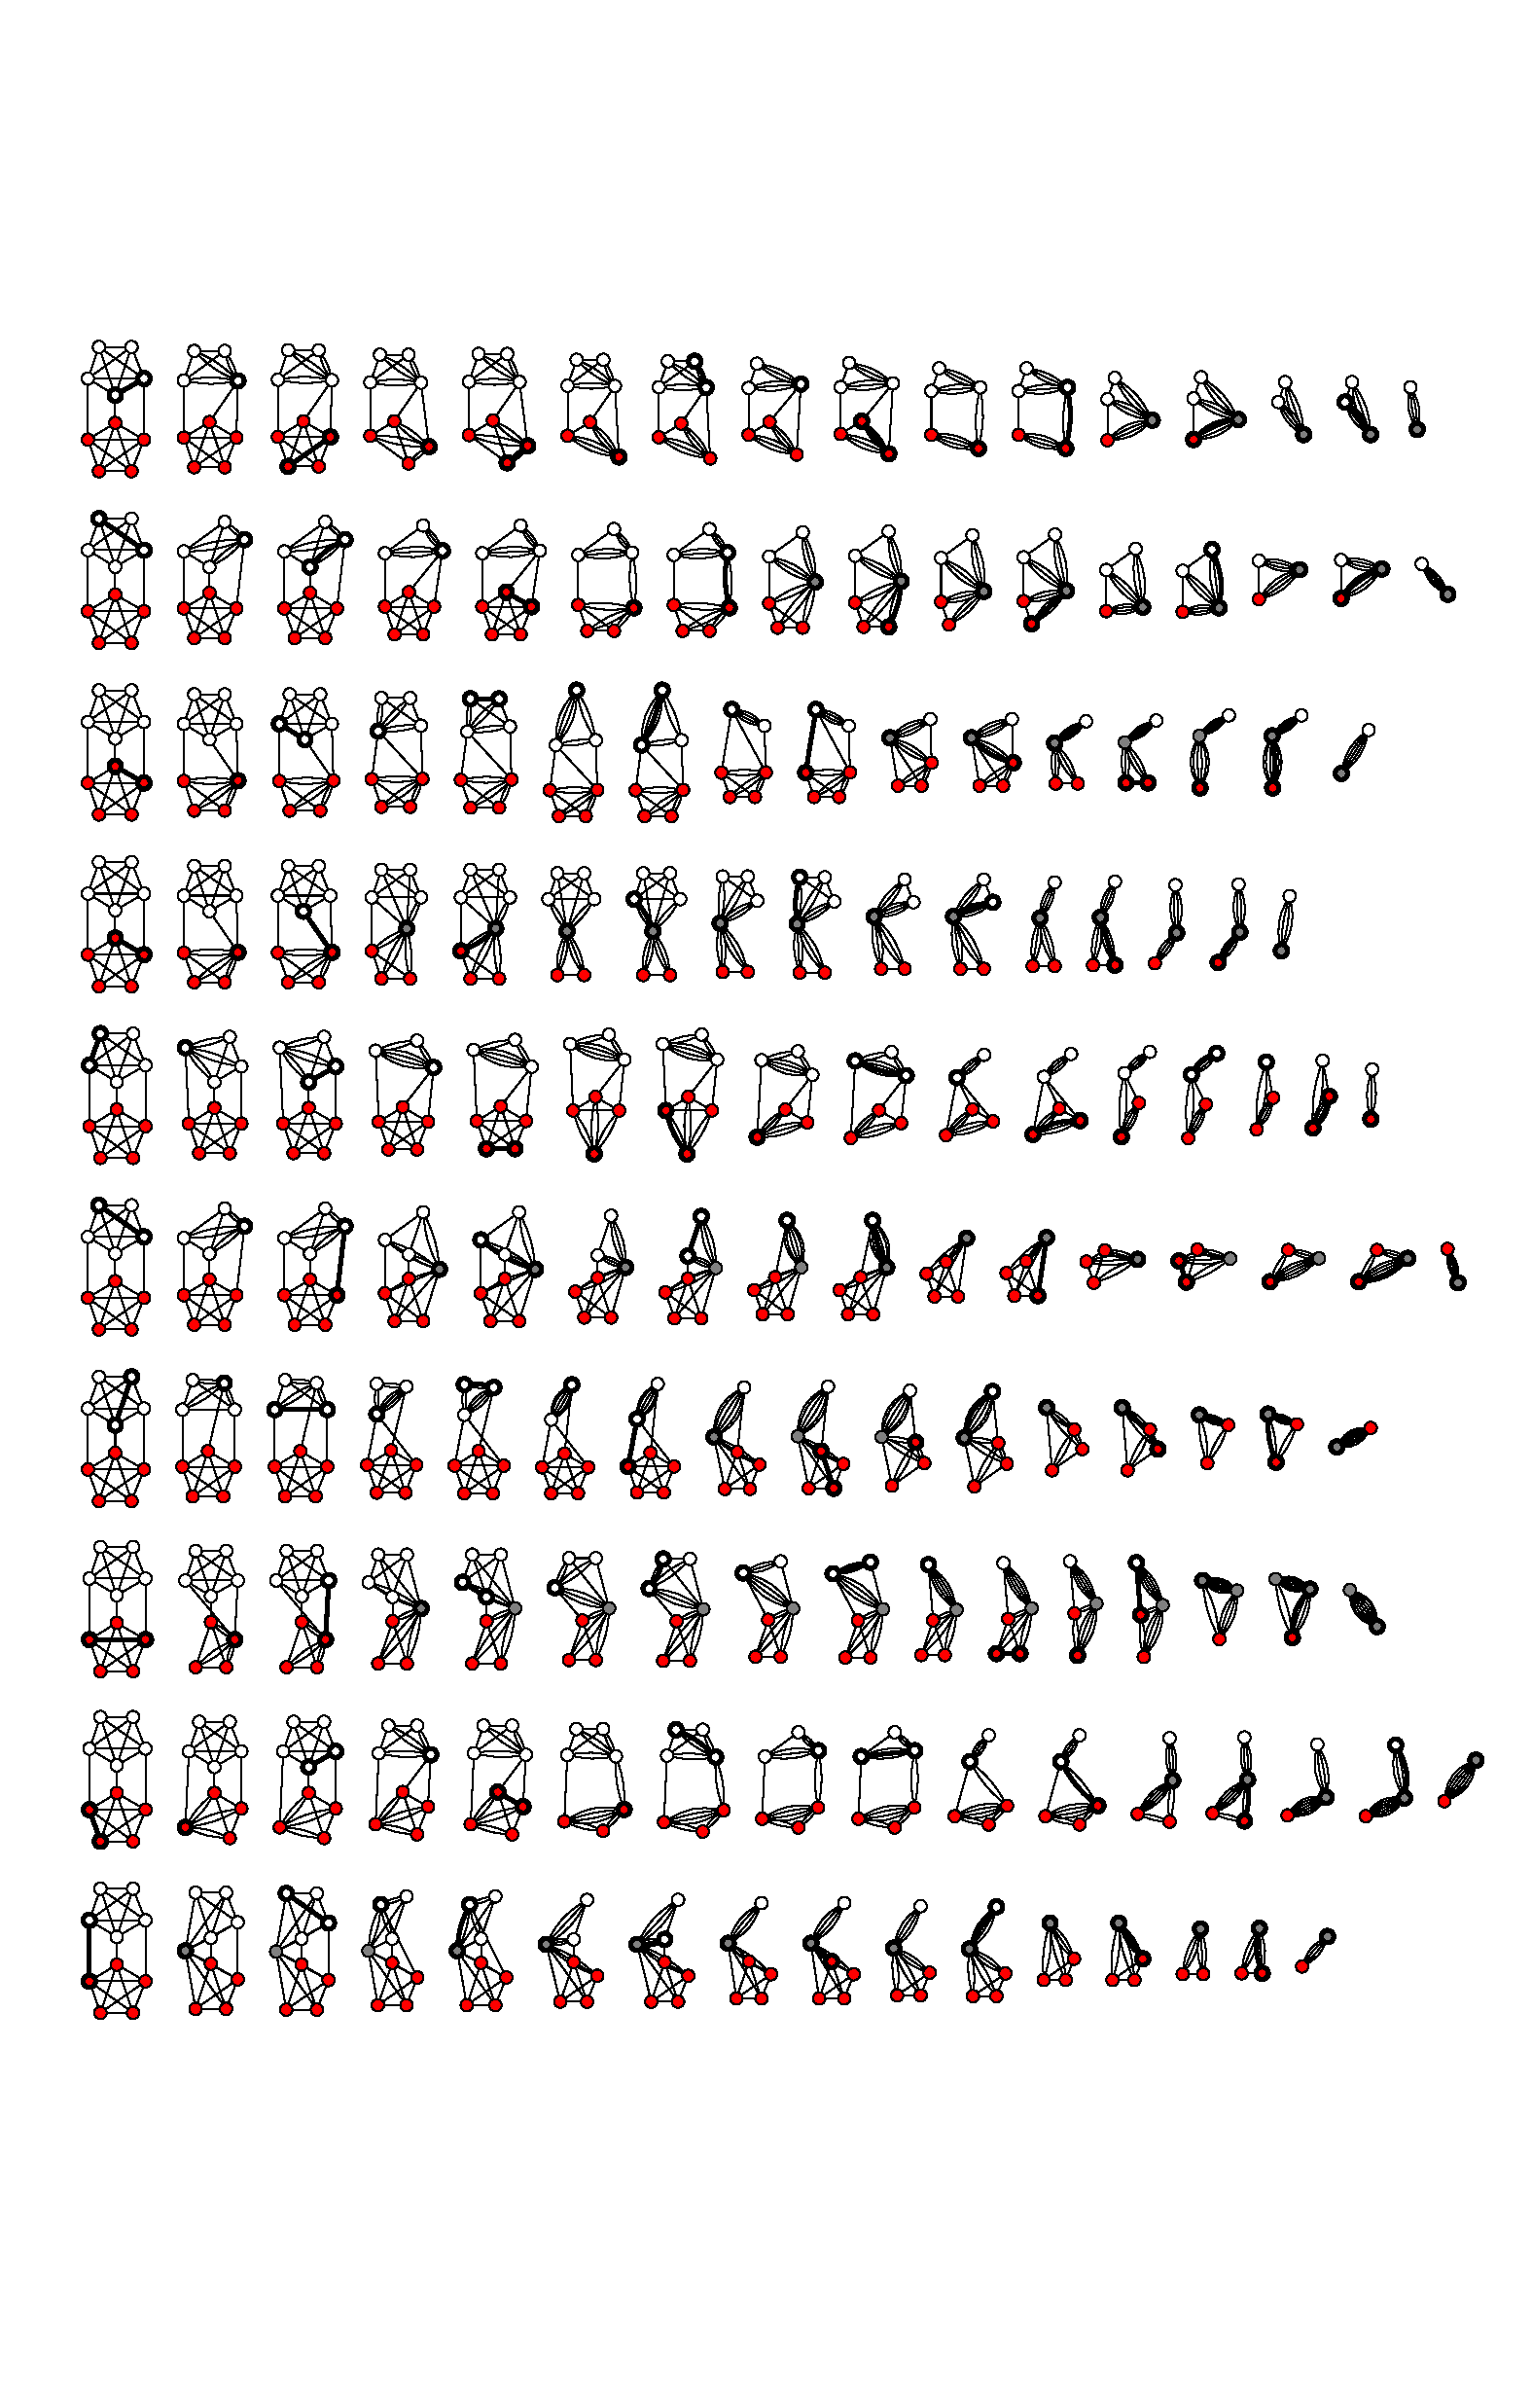
\includegraphics[scale=0.25]{img/kargers.pdf}
\end{frame}
